% https://github.com/martinhelso/phduio-article-based

% Add [final] to remove marginal notes:
%colophon
\documentclass[a4paper, italian]{phduio}

\usepackage{phdstyle}   % Custom style
\usepackage{amsmath}
\usepackage[toc]{glossaries}
\usepackage{mdframed}
%\usepackage[utf8]{inputenc}
\usepackage{caption}
\usepackage{subcaption}
\usepackage{wasysym}
\usepackage{color}
\usepackage{xcolor,colortbl}
\usepackage{tabularx}
\usepackage{array}
\let\newfloat\undefined
\usepackage{floatrow}


\newcommand*{\rom}[1]{\uppercase\expandafter{\romannumeral #1\relax}}

\makeglossaries

\newglossaryentry{latex}
{
    name=latex,
    description={Is a markup language specially suited
for scientific documents}
}

\newglossaryentry{maths}
{
    name=mathematics,
    description={Mathematics is what mathematicians do}
    st Common Multiple
}

\colorlet{shadecolor}{lightgray!50}
\newtheorem{thm-env}{Teorema} % is it right?
\newtheorem{def-env}{Definizione} % is it right?
\newtheorem{ex-env}{Esempio} % is it right?
\newtheorem{prop-env}{Proposizione} % is it right?
\newtheorem{lemma-env}{Lemma} % is it right?
\newenvironment{thm}
{
    \begin{shaded}
    \begin{thm-env}
}
{
    \end{thm-env}
    \end{shaded}
}

\newenvironment{prop}
{
    \begin{shaded}
        \begin{prop-env}
        }
        {
        \end{prop-env}
    \end{shaded}
}

\newenvironment{lemma}
{
    \colorlet{shadecolor}{lightgray!20}
    \begin{shaded}
        \begin{lemma-env}
        }
        {
        \end{lemma-env}
    \end{shaded}
}

\newenvironment{steps}
{
    \begin{enumerate}[label={\emph{Passaggio \arabic*}.}, leftmargin=*]
    }
    {
    \end{enumerate}
}

\newenvironment{definition}
{
    \begin{shaded}
    \begin{def-env}
}
{
    \end{def-env}
    \end{shaded}
}

\newenvironment{example}
{
    \begin{framed}
        \begin{ex-env}
        }
        {
        \end{ex-env}
    \end{framed}
}

%% Custom title page
\newcommand{\unibotitle}
{
    \begin{titlingpage}
        \begin{center}
        {
            \LARGE
            \textsc{Alma Mater Studiorum $\cdot$ Universit\`a di Bologna}
        }
            \rule[0.1cm]{15.8cm}{0.1mm}
            \rule[0.5cm]{15.8cm}{0.6mm}
            \\\vspace{3mm}

            {\small{\textbf{Scuola di Scienze \\
            Dipartimento di Fisica e Astronomia\\\vspace{-.5mm}
            Corso di Laurea in Fisica}}}

        \end{center}

        \vspace{23mm}

        \begin{center}
                {

                    \Huge{
                        \textsc{
                        \centering
                        Applicazione della\\
                         \ Teoria del Controllo:\\
                         \vspace{6mm}
                        \centering
                         \ \ \ il pendolo invertito su rotaia
                        }
                    }
                }\\
        \end{center}

        \vspace{45mm} \par \noindent

        \begin{minipage}[t]{0.47\textwidth}

        {
            \LARGE
            \textbf{Relatore:}
            \vspace{-.75mm}\\
            Professor Armando Bazzani
            \\
            \\

            \textbf{Correlatore:}
            \vspace{2mm}\\
            Dottor Giulio Colombini
            \\
            \\
        }
        \end{minipage}
%
        \hspace{25mm}
        \hfill
%
        \begin{minipage}[t]{0.47\textwidth}
                {
                    \LARGE
                    \textbf{Presentata da:}
                    \vspace{2mm}\\
                    Matteo Bonacini
                }
        \end{minipage}

        \vspace{40mm}

        \begin{center}
            Anno Accademico 2022/2023
        \end{center}

    \end{titlingpage}
}



%\textwidth=450pt\oddsidemargin=0pt



\begin{document}

    \frontmatter        % Folios in Roman numerals, unnumbered chapters.

        \unibotitle % need to replace with unibotitle

        \thispagestyle{empty}
\vspace*{\stretch{1}}
\begin{flushright}
    \emph{To my ghostwriter}
\end{flushright}
\vspace*{\stretch{3}}
        \chapter{Abstract}

pendolo goes swoosh

\section*{Ringraziamenti}

Boh


\vskip\onelineskip
\begin{flushleft}
    \sffamily
    \textbf{Matteo Bonacini}
    \\
    Bologna,\MONTH\the\year
\end{flushleft}

        \cleartorecto
        \tableofcontents    % Or \tableofcontents*
        \cleartorecto
        \listoffigures      % Or \listoffigures*
        \cleartorecto
        \listoftables       % Or \listoftables*
        \cleartorecto
        \printglossary[title=Glossario, toctitle=Glossario]

       \part*{Teoria del controllo: il pendolo invertito su rotaia}
      %  \addcontentsline{toc}{chapter}{\titolo}
       % \cleartorecto

    \mainmatter         % Folios in Arabic numerals, numbered chapters.

            \numberofpapers{5}  % Specify size of thumb indices

            
\title{Introduzione}
\maketitle
\label{sec:intro}


\section{Teoria del Controllo}
La Teoria del Controllo è una disciplina che ha origini antiche,
tracciabili fino all'era degli antichi greci,
%todo cite
e che si è sviluppata formalmente solo nel corso degli ultimi due secoli.
%todo cite, di nuovo

L'obiettivo alla base della Teoria è la necessità di poter alterare
lo stato di un sistema in modo arbitrario, entro i limiti fisici
del sistema stesso.
Anche se per un essere umano questo obiettivo può sembrare banale,
questa è solo un illusione data dall'estrema complessità del cervello umano:
spesso, attività che per noi appaiono semplici, contengono un
alto grado di complessità nascosta.
Basti prendere come esempio \emph{l'atto di andare in bicicletta}.
Un mito comune è che la bicicletta sia \emph{facile} da guidare perchè
è stabilizzata dall'effetto giroscopico delle ruote, che la mantiene in verticale.
Questo è falso!
Uno studio
\cite{bicycle}
%todo cite ALMOST EVERYONE can ride a bicycle, yet apparently no one knows how they do it.
afferma che la bicicletta \emph{deve essere inerentemente instabile} per poter
essere usata da un essere umano; la facilità è data dal nostro cervello che,
in automatico, impara a correggere le instabilità.

I risultati della Teoria si ritrovano in natura in processi di ogni origine.
Dal metabolismo del singolo batterio, ai flussi di automobili nel traffico:
tutto questo necessita di Controllo.
In questa tesi mostrerò alcuni risultati della Teoria e
mostrerò il risultato della loro applicazione ad un vero sistema
meccanico realizzato in laboratorio, il \emph{pendolo (invertito) su rotaia}.

\section{Organizzazione del testo}
Il testo è diviso in cinque capitoli, oltre al presente.
Nei capitoli~\ref{sec:linear-control} e~\ref{sec:nonlinear-control} introduco
i concetti teorici che servono per il mio studio e dimostro alcuni dei risultati
principali della Teoria, applicata ai sistemi lineari e non lineari.
Nel capitolo~\ref{sec:pic} enuncio gli obiettivi del mio studio, sviluppo il modello
teorico del sistema e uso quanto ricavato nei capitoli
precedenti per trovare una strategia di controllo che raggiunga gli obiettivi.
Nel capitolo~\ref{sec:pic-irl} mostro come ho costruito il sistema in laboratorio
e nel capitolo~\ref{sec:results} mostro i risultati che ho ottenuto applicando
il modello teorico al sistema reale.

La trattazione teorica in questo testo è largamente ispirata ai lavori di
Sontag e Brunton.
Nel costo del testo farò uso di altri risultati, che verranno citati di conseguenza.
            \title{Sistemi lineari e controllo}
\maketitle
\label{sec:linear-systems-and-control}



\section{Introduzione}

culo2
\begin{thm}[\text{culo}]
    \label{thm:dedekind}
    Let \( A \) be a Noetherian domain of dimension one. Then the following are equivalent:
    \begin{enumerate}
        \item
        \( A \) is integrally closed;

        \item
        Every primary ideal in \( A \) is a prime power;

        \item
        Every local ring \( A_\mathfrak{p} \) \( (\mathfrak{p} \neq 0) \) is a discrete valuation ring.
    \end{enumerate}
\end{thm}

culo

\section{Controllo ottimale: LQR} \todo glossary
            \title{Controllo non lineare con il metodo di Ljapunov}

\maketitle
\label{sec:nonlinear-control}


\paragraph{Introduzione}

In questo capitolo introduco i concetti di
controllabilità asintotica e di funzione di controllo di
Ljapunov. Dimostro poi il risultato principale
che si ottiene dalle funzioni di Ljapunov, ovvero,
dimostro che trovare una funzione di Ljapunov per un sistema
ne garantisce la controllaiblità.

\input{sections/3/stabilità-asintotica}
\section{Funzioni di controllo di Ljapunov}
Per i sistemi non lineari esiste un criterio che permette di determinarne
la controllabilità asintotica, chiamato \emph{metodo di Ljapunov}.
L'idea è di trovare una \emph{energia generalizzata} $V(\b x)$
che sia sempre decrescente nel tempo,
così che il sistema tenda a minimizzarla.

Per usare i risultati della teoria di Ljapunov è necessario lavorare
in \emph{sistemi topologici}, una classe più ristretta di problemi di controllo.
Per quanto riguarda questo testo è sufficiente pensare a un sistema topologico
come un problema di controllo in cui la mappa di transizione è una funzione
continua.

\begin{definition}
    Un \textbf{sistema topologico} è un problema di controllo in
    cui lo spazio delle fasi $\Sigma$ è dotato di metrica e,
    dato $t \in \mathcal T$ e $\b x \in \Sigma$,
    vale la seguente proprietà:

    Se $\omega$ è un controllo ammesso per $\b x$ e la successione
    ${\b x_n}_n$ tende a $\b x$ allora deve esistere un intero
    $N$ tale che, preso $n \geq N$ allora $\omega$ è ammesso per $x_n$
    e il limite~\eqref{eq:def-sistema-topologico} converge uniformemente a $0$ per $s \in [0, t]$.
    \begin{equation*}
        \lim_{N \to +\infty} d[\phi^s(\b x_n, \omega), \phi^s(\b x, \omega)] = 0.
        \label{eq:def-sistema-topologico}
    \end{equation*}
\end{definition}


Enuncio la definizione di \emph{funzione di controllo di Ljapunov}.
\begin{definition}
    \label{def:clf-local}
    Dato un problema di controllo in cui $\b x^*$ è un punto fisso e
    $\mathcal O$ è un intorno di $\b x^*$.
    Una funzione continua
    \begin{equation*}
        V : \Sigma \to \R,
    \end{equation*}
    $V$ è detta \textbf{funzione locale di controllo di Ljapunov} se
    e solo se valgono le seguenti proprietà:

    \begin{itemize}
        \item 1) $V$ è propria in $\b x^*$, ovvero l'insieme
        \begin{equation*}
            \left\{\b x \in \Sigma\ |\ V(\b x) \leq \epsilon \right\}
        \end{equation*}
        è un sottoinsieme compatto di $\mathcal O$ per ogni $\epsilon$ piccolo a piacere.
        \item 2) $V$ è definita positiva in $\mathcal O$, ovvero $V(\b x^*) = 0$ e
        $V(\b x) > 0$ per ogni $\b x \neq \b x^* \in \mathcal O$.
        \item 3) Per ogni $\b x \neq \b x^* \in \mathcal O$
        esiste un tempo $0 < t \in \mathcal T$ e un controllo $\omega \in \mathcal U^{[0,t[ \subseteq \mathcal T}$
        tali che, detta $\xi(s) = \phi^s(\b x, \omega)$,
        \begin{align*}
            V(\xi(s)) &\leq V(\b x) \text{ per ogni } s \in [0,t[ \subseteq \mathcal T, \\
            V(\xi(t)) &< V(\b x).
        \end{align*}
    \end{itemize}
\end{definition}

\begin{definition}
    Se nella definizione~\ref{def:clf-local} l'intorno $\mathcal O$ coincide
    con tutto lo spazio delle fasi $\Sigma$ allora $V$ è una
    \textbf{funzione di controllo di Ljapunov}.
    \label{def:clf}
\end{definition}

Le definizioni~\ref{def:clf-local} e~\ref{def:clf} valgono anche per sistemi
senza controlli; in questo caso $V$ è chiamata solamente "\emph{funzione (locale) di Ljapunov}".
Il termine "(\emph{locale})" tra parentesi indica che l'affermazione è da intendersi valida
sia che il termine "\emph{locale}" sia presente o meno.

\begin{definition}
    Sia $V$ una funzione (locale) di controllo di Ljapunov.
    Dati $\b x, \b z \in \Sigma$, si dice che $\b z$ è \textbf{ben raggiungibile
    da} $\b x$ se esiste un tempo $t > 0$ e un controllo $\omega \in \mathcal U^{[0,t[ \subseteq \mathcal T}$ ammesso per $\b x$
    tale che per $\xi(s) = \phi^s(\b x, \omega)$ con $\xi(t) = \b z$, vale
    \begin{align*}
        V(\xi(s)) &\leq V(\b x) \text{ per ogni } s \in ]0,t[ \subseteq \mathcal T, \\
        V(\xi(t)) &< V(\b x).
    \end{align*}
    \label{def:ben-raggiungibile}
\end{definition}

Enuncio il risultato principale che si ottiene dalle funzioni di Ljapunov.
\begin{thm}
    Dato un sistema topologico, se esiste una funzione (locale) di controllo di Ljapunov,
    allora il problema è (localmente) asintoticamente controllabile.
    \label{thm:ljapunov}
\end{thm}

\emph{Dimostrazione}.
La dimostrazione si basa sulla costruzione di una strategia di
controllo che porti il sistema verso $\b x^*$ in un tempo infinito.
Per chiarezza, divido la dimostrazione in più passaggi; dimostro prima la versione locale
del teorema e poi quella globale.
\begin{steps}
    \item Grazie alla prorpietà (1) della definizione~\ref{def:clf-local}
    posso scegliere un numero $\alpha_0$ tale che l'insieme
    \begin{equation}
        C = \left\{ x\ |\ V(x) \leq \alpha_0 \right\} \subset \mathcal O
        \label{eq:alpha_0}
    \end{equation}
    sia \emph{compatto}.

    Dimostro la seguente affermazione

    \begin{aff}
        Per ogni intorno aperto $\mathcal W$ di $\b x^*$ esiste
        un $\beta > 0$ tale che
        \begin{equation*}
            \{\b x\ |\ V(\b x) \leq \beta\} \subset \mathcal W.
        \end{equation*}
    \end{aff}

    \emph{Dimostrazione}.
    Procedo per assurdo.
    Se così non fosse, esisterebbe una sequenza di elementi di $\Sigma$
    \begin{equation*}
    \{\b x_n\}_n
    \end{equation*}
    tali che comunque preso $n$, $\b x_n \notin \mathcal W$ e
    \begin{equation*}
        V(\b x_n) \to 0 \text{ per } n \to +\infty.
    \end{equation*}
    Senza perdere di generalità, assumo che tutti gli $\b x_n$
    siano contenuti in $K$, dato da
    \begin{equation*}
        K = \bar{\mathcal W} \bigcap C
    \end{equation*}
    dove $\bar{\mathcal W}$ indica il complementare di $\mathcal W$.
    La costruzione per la dimostrazione è mostrata in figura~\ref{fig:ljapunov-dim-aff1}.

    \hfill
    \begin{minipage}{.8\textwidth}
        \begin{figure}[H]
            \centering
            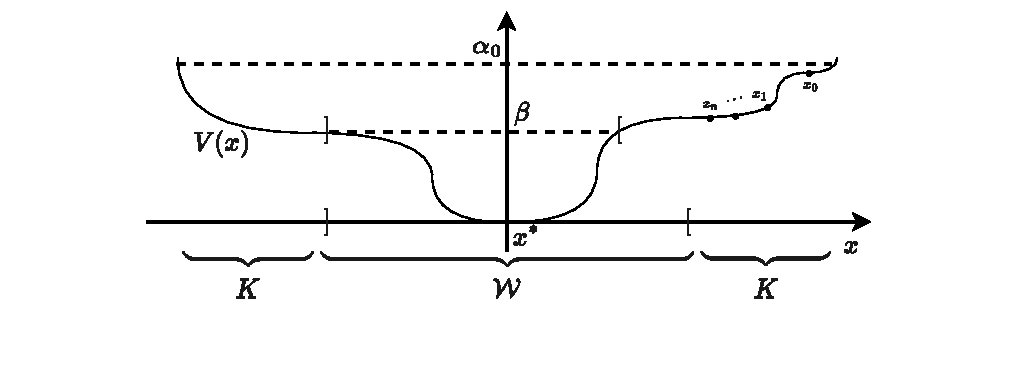
\includegraphics[width=\textwidth]{assets/ljapunov-dim-aff1}
            \caption[Costruzione 1 per teorema di Ljapunov]{Costruzione per dimostrare
            l'affermazione 1.}
            \label{fig:ljapunov-dim-aff1}
        \end{figure}
    \end{minipage}

    Per il teorema di Bolzano-Weierstrass, posso estrarre una
    sottosuccessione di $\{\b x_n\}_n$ convergente in $K$
    \begin{equation*}
    \{\b x_n\}_k \to \b x.
    \end{equation*}
    Ma per la continuità do $V$ vale
    \begin{equation*}
        V(\b x) = 0
    \end{equation*}
    e dalla proprietà (2) della definizione~\ref{def:clf-local}
    segue che
    \begin{equation*}
        \b x = \b x^*.
    \end{equation*}
    Ma questo è un assurdo, visto che che $\b x \in K$
    e $\b x^* \in \mathcal W \subset \bar K$, provando l'affermazione.

    \hfill\openbox\paragraph{}

    Una conseguenza utile dell'affermazione (1) è che se
    $\xi(t) = \phi^t(\b x, \omega)$ con $t \in [0, +\infty[$ tale che
    \begin{equation*}
        V[\xi(t)] \to 0 \text{ per } t \to +\infty
    \end{equation*}
    allora deve essere
    \begin{equation}
        \xi(t) \to \b x^*.
        \label{eq:xi-to-xstar}
    \end{equation}


    \item Osservo che la proprietà (3) della definizione~\ref{def:clf-local}
    garantisce che per ogni stato $\b y \in \mathcal O$ e $\b y \neq \b x^*$ esiste
    almeno uno stato ben raggiungibile da $\b y$.
    Inoltre vale la proprietà transitiva, ovvero, se $\b y$ è raggiungibile da $\b x$
    e $\b z$ è raggiungibile da $\b y$, allora $\b z$ è raggiungibile da $\b x$.
    Definisco
    \begin{equation*}
        B(\b x) = \inf\left\{ V(\b z)\ |\ \b z \text{ è ben raggiungibile da } \b x \right\}
    \end{equation*}
    e osservo che, per quanto appena detto, vale che $B(x) < V(x)$ per $x \neq \b x^*$.
    Dimostro la seguente affermazione.

    \begin{aff}
        \begin{equation*}
            V(\b x) < \alpha_0 \implies B(\b x) = 0,
        \end{equation*}
        dove $\alpha_0$ definisce un insieme compatto, secondo la~\eqref{eq:alpha_0}.
    \end{aff}

    \emph{Dimostrazione}.
    Procedo per assurdo.
    Suppongo che esista un $\b x \neq \b x_0$ per cui $V(\b x) < \alpha_0$
    e $B(\b x) = \alpha > 0$.
    Per come ho scelto $\alpha_0$ deve valere $\b x \in \mathcal O$.
    Considero la successione\footnote{L'esistenza
    è garantita dalla proprietà transitiva della ben raggiungibilità e dal fatto che
    ogni $z_n$ ha almneno un elemento che è ben raggiungibile.}
    \begin{equation}
        \{V(\b z_n)\}_n
        \label{eq:successione-zn}
    \end{equation}
    decrescente dove gli $\b z_n$ sono tutti elementi ben raggiungibili da $\b x$.
    La~\eqref{eq:successione-zn} è limitata da $V(\b z) = \alpha$.
    Tutti gli $\b z_n$ fanno parte del compatto
    \begin{equation*}
        C = \left\{\b z \ |\ V(\b z) \leq V(\b x) \right\}
    \end{equation*}
    e dato che la~\eqref{eq:successione-zn} è monotona e limitata,
    allora è anche convergente e posso fissarne il limite senza perdere
    di generalità:
    \begin{equation}
        \lim_{\b z_n \to \b z} V(\b z_n) = V(\b z) = \alpha.
        \label{eq:vzequalsalpha}
    \end{equation}
    Osservo che
    \begin{equation*}
        \alpha \neq 0 \implies z \neq \b x^*
    \end{equation*}
    e che
    \begin{equation*}
        \alpha < V(\b x) < \alpha_0 \implies \b z \in \mathcal O.
    \end{equation*}
    Quindi, deve esistere un $\b y$ che sia ben raggiungibile da $\b z$.
    È importante osservare che, anche se ogni elemento della successione~\eqref{eq:successione-zn}
    è ben raggiungibile da $\b x$, non ho nulla che mi garantisca che $\b z$ lo sia.
    Fisso $\epsilon > 0$ tale che
    \begin{equation}
        V(\b z) < V(\b x) - \epsilon,\ \text{e} \ V(\b y) < V(\b z) - \epsilon
        \label{eq:vy-less-vz}
    \end{equation}
    e prendo $\nu \in \mathcal U^{[0, t[ \subseteq \mathcal T}$ controllo ammesso
    per $\b z$ tale che, detto $\zeta(s) = \phi^s(\b z, \nu)$, valgano
    \begin{align*}
        &\zeta(t) = \b y, \\
        V(&\zeta(s)) \leq V(\b z), \ \forall s \in [0, t[ \subseteq \mathcal T.
    \end{align*}
    La costruzione per la dimostrazione è mostrata in figura~\ref{fig:ljapunov-dim-aff2}.

    \hfill
    \begin{minipage}{.8\textwidth}
        \begin{figure}[H]
            \centering
            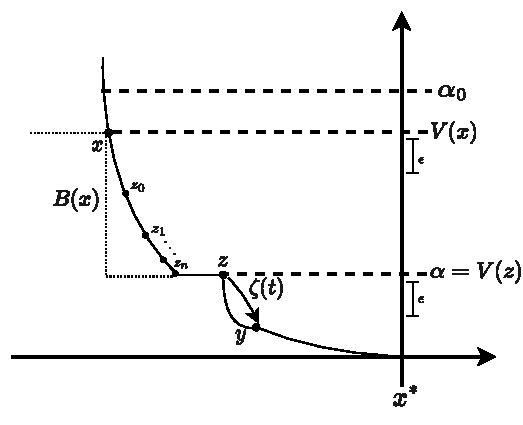
\includegraphics[width=.5\textwidth]{assets/ljapunov-dim-aff2}
            \caption[Costruzione 2 per teorema di Ljapunov]{Costruzione per dimostrare
            l'affermazione 2.}%todo
            \label{fig:ljapunov-dim-aff2}
        \end{figure}
    \end{minipage}

    $V$ è uniformemente continua\footnote{Per ipotesi
        $V$ e continua sul compatto $C$ quindi per il teorema di Heine-Cantor è
        uniformemente continua su $C$.} sul compatto $C$ quindi, fissato $\epsilon >0$ esiste un $\delta > 0$
    tale che, presi $\b a, \b b \in C$
    \begin{equation}
        d(\b a, \b b) < \delta \implies |V(\b a) - V(\b b)| < \epsilon.
        \label{eq:v-uniformemente-continua}
    \end{equation}

    Considero la successione
    \begin{equation*}
        \{V(\b y_n)\}_n,\ \b y_n = \zeta_n(t)
    \end{equation*}
    con $\zeta_n(s) = \phi^s(\b z_n, \nu)$.

    Visto che sto lavorando su uno spazio topologico vale\footnote{Per la continuità
    della mappa di transizione} che, fissato $\epsilon > 0$, esiste $\delta > 0$ tale che,
    per valori $n \geq N$ vale
    \begin{equation}
        d_\infty(\zeta_n, \zeta) < \delta \implies d(\b y_n, \b y) < \epsilon,
        \label{eq:phi-continua}
    \end{equation}
    dove $d_\infty$ è la metrica per lo spazio dei controlli ammessi definita da
    \begin{equation*}
        d_{\infty}[\phi^t(\b x, \omega_1), \phi^t(\b x, \omega_2)] =
        \sup \left\{ d[\phi^s(\b x, \omega_1), \phi^s(\b x, \omega_2)],\ s \in \mathcal T  \right\}.
    \end{equation*}
    Ora fisso $\epsilon > 0$ e considero la catena di implicazioni data
    dalla~\eqref{eq:v-uniformemente-continua} e dalla~\eqref{eq:phi-continua}:
    \begin{equation}
        d_\infty(\zeta_n, \zeta) < \delta' \implies d(\b y_n, \b y) < \delta \implies |V(\b y_n) - V(\b y)| < \epsilon
        \label{eq:implication-chain}
    \end{equation}
    da cui
    \begin{equation}
        \left| V[\zeta_N(s)] - V[\zeta(s)] \right| < \epsilon\ \forall s \in [0, t].
        \label{eq:lesser-forall-t}
    \end{equation}

    Dimostro che $\b y_N$ è ben raggiungibile da $\b x$.
    È sufficiente dimostrare che
    \begin{equation*}
        V[\zeta_N(s)] < V(\b x) \forall s \in [0, t].
    \end{equation*}
    Considero la~\eqref{eq:lesser-forall-t} e applico la definizione di modulo.
    \begin{itemize}
        \item Caso $V[\zeta(s)] < V[\zeta_N(s)]$.
            \begin{align*}
                V[\zeta_N(s)] - V[\zeta(s)] &< \epsilon \\
                V[\zeta_N(s)] &< \epsilon + V[\zeta(s)] \\
                V[\zeta_N(s)] &< \epsilon + V(\b z) \\
                V[\zeta_N(s)] &< V(\b x) \numberthis\label{eq:modulo-caso-1}
            \end{align*}
            dove nell'ultimo passaggio ho applicato la~\eqref{eq:vy-less-vz}.
        \item Caso $V[\zeta(s)] > V[\zeta_N(s)]$.
            \begin{align*}
                V(\b x) > V(\b z) > V[\zeta(s)] > V[\zeta_N(s)]. \numberthis\label{eq:modulo-caso-2}
            \end{align*}
    \end{itemize}
    Chiamo $\omega$ la legge di controllo che porta $\b x$ a $\b z_N$.
    Per la proprietà di composizione della mappa di transizione, posso concatenare
    $\omega$ con $\nu$, in modo da ottenre una legge di controllo che porta $\b x$ a $\b y_N$.
    Questo, unito al fatto che la~\eqref{eq:modulo-caso-1} e la~\eqref{eq:modulo-caso-2}
    valgono per $s \in [0, t]$, è sufficiente a dimostrare che $\b y_N$ è ben raggiungibile da $\b x$.

    In questo modo cado in assurdo visto che la~\eqref{eq:implication-chain}
    unita alla~\eqref{eq:vy-less-vz} e alla~\eqref{eq:vzequalsalpha} implicano
    che $V(\b y_n) < B(\b x)$, violando la tesi.
    L'assurdo è dato dall'aver assunto che $\alpha = B(\b x) > 0$.

    \hfill \openbox \paragraph{}

    L'andamento di $B(\b x)$ è mostrato in figura~\ref{fig:ljapunov-aff2}.

    \hfill
    \begin{minipage}{.8\textwidth}
        \begin{figure}[H]
                \centering
                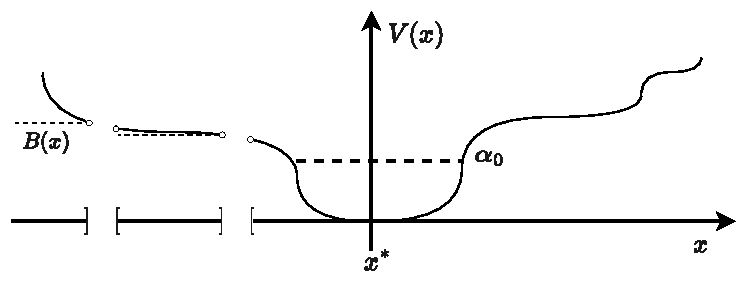
\includegraphics[width=\textwidth]{assets/ljapunov-aff2}
                \caption[Andamento di $B(\b x)$]{Andamento di $B(x)$ per uno
                spazio delle fasi monodimensionale. La funzione è a tratti e
                si annulla dentro al compatto più grande contenente $x^*$.}
                \label{fig:ljapunov-aff2}
        \end{figure}
    \end{minipage}

    \item Dimostro che vale la seguente affermazione

    \begin{aff}
        Se $V(\b x) < \alpha_0$ con $\b x \neq \b x^*$ allora esiste
        una sequenza di stati
        \begin{equation*}
        \{\b x_n\}_{n\geq0}
        \end{equation*}
        con $\b x_0 = \b x$, una sequenza di tempi
        \begin{equation*}
        t_n \in \mathcal T
        \end{equation*}
        e una sequenza di controlli
        \begin{equation*}
            \omega_n \in \mathcal U^{[0, t_n[ \in \mathcal T}
        \end{equation*}
        tale che valgano le seguenti proprietà
        \begin{itemize}
            \item $\omega_n$ è ammesso per $\b x_n$.
            \item $\phi^{t_n}(\b x_n, \omega_n) = \b x_{n+1}$
            \item Con $\xi_n(t) = \phi^t(\b x_n, \omega_n)$ vale $V[\xi_n(t)] \leq \frac 1 {2^n} V(\b x), \ \forall t \in [0, t_n]$
        \end{itemize}
    \end{aff}
    \emph{Dimostrazione}.
    Procedo per induzione.
    Voglio dimostrare che  per ogni $\b x \in \Sigma$ tale che
    \begin{equation*}
        0 < V(\b x) < \alpha_0
    \end{equation*}
    esiste un certo tempo $t > 1$ e un controllo $\omega$
    di lunghezza $t$ ammesso per $\b x$ tale che
    \begin{align*}
        V[\xi(s)] &\leq V(\b x) \text{ con } s \in [0, t], \\
        V[\xi(t)] &< \frac 1 2 V(\b x).
    \end{align*}
    Per continuità di $V$ in $\b x^*$, esiste un $\epsilon > 0$ per cui
    \begin{equation}
        d(\b z, \b x^*) < \epsilon \implies V(\b z) < \frac 1 2 V(\b x).
        \label{eq:dzxstar}
    \end{equation}
    Sia $\omega_0 \in \mathcal U^{[0, 1[}$ il controllo nullo,
    tale che
    \begin{equation*}
        \phi^s(\b x^*, \omega_0) = \b x^*.
    \end{equation*}
    Visto che sto lavorando in uno spazio topologico
    esiste un $\delta > 0$ tale che, fissato $\epsilon > 0$ e
    dato $\zeta(s) = \phi^s(\b y, \omega_0)$,
    \begin{equation*}
        d(\b y, \b x^*) < \delta \implies d(\zeta(s), \b x^*) < \epsilon
    \end{equation*}
    e $\omega_0$ è ammesso per $\b y$ per $s \in \mathcal T$.

    Per la~\eqref{eq:dzxstar} posso scegliere $\epsilon$ in modo che
    \begin{equation*}
        V[\zeta(s)] < \frac 1 2 V(\b x)
    \end{equation*}
    valga per $s \in [0, 1]$.
    Per l'affermazione (1) esiste $\delta_0 > 0$ tale che
    \begin{equation}
        V(\b y) < \delta_0 \implies d(\b y, \b x^*) < \delta.
        \label{eq:vylessdelta0}
    \end{equation}
    Per l'affermazione (2), vale $B(\b x) = 0$.
    Quindi esiste un controllo $\omega_1$ e un tempo $t_1$ tale
    che, dato $\xi_1 = \phi^{t_1}(\b x, \omega_1)$, vale
    \begin{align*}
        V[\xi_1(s)] &\leq V(\b x), \text{ con } s \in [0, t_1],\\
        V[\xi_1(t_1)] &< \delta_0
    \end{align*}
    e, per la~\eqref{eq:vylessdelta0}, vale anche
    \begin{equation*}
        d[\xi_1(t_1), \b x^*] < \delta.
    \end{equation*}
    La costruzione per la dimostrazione è mostrata in figura~\ref{fig:ljapunov-dim-aff3}.

    \hfill
    \begin{minipage}{.8\textwidth}
        \begin{figure}[H]
            \centering
            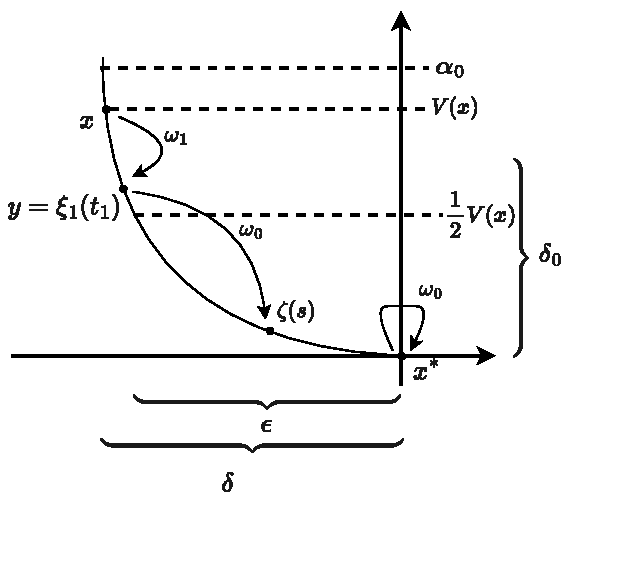
\includegraphics[width=.6\textwidth]{assets/ljapunov-dim-aff3}
            \caption[Costruzione 3 per teorema di Ljapunov]{Costruzione per dimostrare
            l'affermazione 3.}%todo
            \label{fig:ljapunov-dim-aff3}
        \end{figure}
    \end{minipage}

    La sequenza che cerco è quindi data dalla concatenazione di
    $\omega_1$ e $\omega_0$ opportunamente traslati.

    \hfill\\openbox\paragraph{}

    L'affermazione (3) mi permette di definire una legge di controllo
    $\omega$ su $[0, +\infty[ \subseteq \mathcal T$ ammessa per $\b x$
    data dalla concatenazione degli $\omega_n$.
    Detta quindi $\xi(t) = \phi^t(\b x, \omega)$ vale
    \begin{equation*}
        V[\xi(t)] \to 0 \text{ per } t \to +\infty
    \end{equation*}
    e per la~\eqref{eq:xi-to-xstar} vale
    \begin{equation}
        \xi(t) \to \b x^*.
        \label{eq:xi-to-xstar-2}
    \end{equation}

    \item Dimostro che il sistema è localmente asintoticamente
    controllabile.
    Prendo $\mathcal V$ un intorno di $\b x^*$, prendo $\alpha_1$ tale che
    \begin{equation}
     \{\b y\ |\ V(\b y) < \alpha_1 \} \subseteq \mathcal V
        \label{eq:def-alpha1}
    \end{equation}
    e definisco
    \begin{equation*}
        \alpha = \min\{\alpha_0, \alpha_1\}.
    \end{equation*}
    Nella definizione di localmente asintoticamente controllabile prendo
    \begin{equation*}
            \mathcal W = \{\b y\ |\ V(\b y) < \alpha\}.
    \end{equation*}

    L'affermazione (3) è valida per ogni $\b y \neq \b x^* \in \mathcal W$
    dato che $V(\b y) < \alpha_0 \leq \alpha$.
    Quindi, per la~\eqref{eq:xi-to-xstar-2} esiste un controllo $\omega$
    su $\mathcal T$ tale che
    \begin{align*}
        \phi^0(\b y, \omega) = \b y, \\
        \phi^t(\b y, \omega) \to \b x^* \text{ per } t \to +\infty
    \end{align*}
    e per la~\eqref{eq:def-alpha1} vale anche
    \begin{equation*}
        \phi^t(\b y, \omega) \in \mathcal V, \ t \in [0, +\infty[ \subseteq \mathcal T.
    \end{equation*}
    quindi il sistema è localmente asintoticamente controllabile.

    \hfill\qedsymbol\paragraph{}

    \item Dimostro che il sistema è asintoticamente controllabile.
    Assumo che $V$ sia una funzione di controllo di Ljapunov globale
    e prendo $\b y \in \Sigma$.
    Sia $\beta = V(\b y)$.
    Ora osservo che nella dimostrazione fatta fino ad ora posso prendere
    $\mathcal O = \Sigma$ e $\alpha_0 = \beta + 1$
    senza perdere di generalità, in quanto l'unica proprietà che $\mathcal O$
    e $\alpha_0$ devono rispettare è che l'insieme $C$
    definito nella~\eqref{eq:alpha_0}
    sia compatto e contenuto sin $\mathcal O$.
    Quindi, se nel passaggio (4) prendo $\mathcal V = \Sigma$
    posso prendere $\alpha_1 = \beta + 1$ in modo che
    $\b y \in \mathcal{W}$ e che il sistema sia
    asintoticamente controllabile a $\b x^*$.

    \hfill\qedsymbol\paragraph{}



\end{steps}



            \title{Pendolo invertito su rotaia}
\maketitle
\label{sec:pic}


\section{Introduzione}
\paragraph{Il pendolo invertito su rotaia è un sistema facile da modellare,}
ma presenta alcune caratterische che rendono interessante studiarne la controllabilità.
Il sistema è mostrato in figura \ref{fig:pic} e consiste in un pendolo rigido, libero di ruotare e vincolato a muoversi lungo una rotaia rettilinea tramite un carrello. L'unico modo in cui i sistema può interagire con l'esterno è tramite una forza applicata sul carrello lungo la direzione della rotaia. Quando il pendolo è fermo ed è diretto verso l'alto, si trova in un punti di equilibrio instabile e ogni minima perturbazione tenderà a farlo ricadere verso il basso. L'obiettivo che mi pongo è duplice:

\begin{enumerate}
    \item Stabilizzare il pendolo attorno al punto di equilibrio instabile, in modo che sia resistente alle perturbazioni.
    \item Trovare una strategia per portare il pendolo in prossimità del punto di equilibrio instabile, partendo dalla configurazione stabile (\emph{swing-up}).
\end{enumerate}

%todo traduci in italiano
\paragraph{Il sistema è non-lineare e underactuated.} Questo significa che per portare a termine i due obiettivi discussi sopra, è necessario unire le due strategie di controllo discusse nei capitoli \ref{sec:linear-control}  e \ref{sec:nonlinear-control}. Inoltre, un singolo input deve essere in grado di controllare un sistema a due gradi di libertà: la posizione del carrello e l'angolo del pendolo, rientrando nei limiti di lunghezza della rotaia. In questo paragrafo creerò un modello del sistema e lo userò sia per dimostrare che è possibile effettuare lo swing-up del pendolo, sia per disegnare controller LQR per stabilizzarlo. Mostrerò quindi che è possibile raggiungere l'obiettivo che mi sono posto mettendo assieme le due strategie di controllo. Per concludere, userò il modello per stimare alcuni parametri del sistema reale.

%todo
\begin{figure}[thb]
    \centering
    %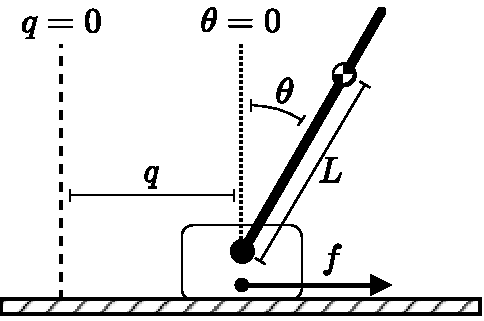
\includegraphics[width=0.4\textwidth]{assets/pic.png}
    \caption{Pic system. Qui ci va tutta la figura e la descrizione del sistema. }%todo
    \label{fig:pic}
\end{figure}
\section{Modello del sistema}
Il sistema consiste in un pendolo rigido, libero di ruotare e vincolato a muoversi lungo una rotaia rettilinea tramite un carrello.
L'unico controllo che ho sul sistema è
una forza applicata sul carrello lungo la direzione della rotaia,
così come è mostrato in figura~\ref{fig:pic}.
Io sono interessato
ad applicare questo studio nel mondo reale, quindi devo tenere
in considerazione che la forza è generata da un motore in risposta
a un segnale di input.
Il motore che prendo in considerazione è un motore elettrico
spazzolato. Visto che il motore è un sistema dinamico in sé,
è conveniente modellarlo separatamente rispetto al sistema
carrello-pendolo.
In figura~\ref{fig:pic-real} è
mostrato uno schema del sistema reale.

\begin{figure}[h]
    \centering
    \begin{subfigure}[b]{0.4\textwidth}
        \centering
        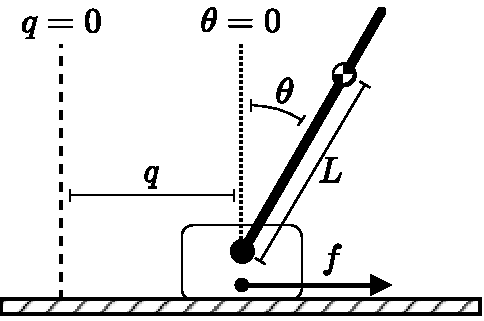
\includegraphics[width=\textwidth]{assets/pic}
        \caption{Schema ideale del sistema. La forza di controllo esterna
        agisce direttamente sul carrello, nella direzione dello scorrimento.}
        \label{fig:pic}
    \end{subfigure}
    \hfill
    \begin{subfigure}[b]{0.48\textwidth}
        \centering
        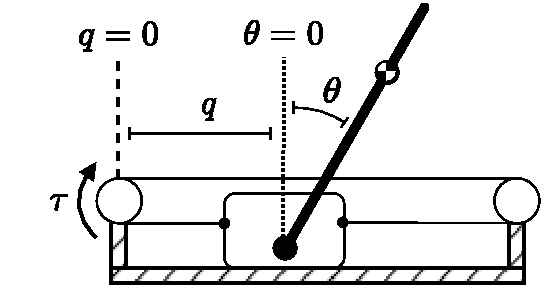
\includegraphics[width=\textwidth]{assets/pic-real}
        \caption{Schema reale del sistema. La forza di controllo viene
        generata da un motore e trasferita al carrello con una cinghia.}
        \label{fig:pic-real}
    \end{subfigure}
    \caption{Schema del sistema ideale e reale. Nelle figure sono mostrate le variabili
    utilizzate.}
\end{figure}



\subsection{Pendolo e carrello}
Riporto i parametri e le variabili d'interesse per il sistema in 
tabella~\ref{tab:parametri} e ricavo le equazioni del moto
usando l'approccio Lagrangiano.
Energia cinetica e potenziale sono
\begin{align*}
        T &= \frac 1 2 M  \dot q^2 + \frac 1 2 m v_{cm}^2 + \frac 1 2 (I - lm^2)\dot \theta^2, \\ %todo
        V &= mgL \cos\theta
\end{align*}
dove $v_{cm}$ è la velocità del centro di massa del pendolo, data da
\begin{equation*}
    v^2_{cm} = (\dot x + l \dot \theta \cos \theta)^2 + (+ l \dot \theta \sin \theta)^2.
\end{equation*}




%todo here
Scrivo la Lagrangiana del sistema
\begin{equation*}
    \mathcal L = T - V
\end{equation*}
e imposto le equazioni di Eulero-Lagrange:

\begin{equation}
        \left\{
        \begin{aligned}
            \totald t \partiald{\dot q} {\mathcal L} - \partiald q {\mathcal L} &= f \\
            \totald t \partiald{\dot \theta} {\mathcal L}  - \partiald \theta {\mathcal L} &= 0
        \end{aligned}
        \right.
        \label{eq:eulero-lagrange-pendolo}
\end{equation}
in cui trascuro gli attriti tra carrello e rotaia e tra
pendolo e perno.
Dal sistema~\eqref{eq:eulero-lagrange-pendolo} ricavo le equazioni del moto:
\begin{equation}
        \left\{
        \begin{aligned}
            \ddot x &= \frac {-lm \ddot \theta \cos \theta + lm \dot \theta^2 \sin \theta + f} {m + M} \\
            \ddot \theta &= \frac {lm (g\sin \theta - \cos \theta) }{I} \ddot x
        \end{aligned}
    \right.
    _.
    \label{eq:moto-sistema}
\end{equation}
Concludo studiando i punti di equilibrio del sistema.
L'unica variabile che compare nel potenziale è $\theta$; impongo
\begin{equation*}
    \left. \frac \partial {\partial \theta}\right |_{V=V_{eq}} V =  0
\end{equation*}
da cui
\begin{equation*}
     V_{eq} = \{0, \pi\}.
\end{equation*}
La stabilità è data da considerazioni fisiche
\begin{align*}
    \theta &= 0  \text{ è instabile}, \\
    \theta &= \pi  \text{ è stabile}.
\end{align*}

\bgroup
\renewcommand{\tabularxcolumn}[1]{>{\arraybackslash}m{#1}}
\renewcommand\arraystretch{1.5}
\begin{table}[h]
    \centering
    \begin{tabularx}{\textwidth}{| gc | X |}
        \noalign{\hrule height 2pt}

        \rowcolor{Black}%

        \multicolumn{1}{=c}{\rowstyle{\bfseries\sffamily \color{White}} Parametro/Variabile} & \multicolumn{1}{+c}{ Descrizione} \\
        \hline
        $g$ & Accelerazione di gravità. \\
        \hline
        $M$ & Massa del carrello. \\
        \hline
        $m$ & Massa del pendolo. \\
        \hline
        $L$ & Distanza tra il centro di massa del pendolo e il punto di rotazione. \\
        \hline
        $I$ & Momento d'inerzia del pendolo calcolato rispetto al punto di rotazione. \\
        \hline
        $q$ & Posizione del carrello rispetto all'origine. \\
        \hline
        $\theta \in ]-\pi, +\pi]$ & Angolo del pendolo rispetto alla verticale. \\
        \hline
        $f$ & Forza agente sul carrello. \\
        \noalign{\hrule height 2pt}
    \end{tabularx}
    \caption{Descrizione di parametri e variabili del sistema carrello-pendolo.}
    \label{tab:parametri}
\end{table}
\egroup

\subsection{Motore}
\todo{fix reference}
%{https://homepages.laas.fr/lzaccari/seminars/DCmotors.pdf}
Lavoro con un motore \textsc{DC} spazzolato.
Riporto i parametri e le variabili d'interesse per il motore in tabella~\ref{tab:parametri-motore}.
Si può ricavare che valgono le equazioni
\begin{subequations}
    \begin{empheq}[left=\empheqlbrace,right=_.]{align}
            u &= L_a \dot J + R_a J + K_e \omega \label{eq:motore-1} \\
            \tau &= K_m J \label{eq:motore-2}
    \end{empheq}
\end{subequations}

Voglio ricavare la forza esercitata dal motore in funzione di $u$.
Dalla~\eqref{eq:motore-2} ricavo
\begin{equation}
        \dot J = \totald t \left( \frac \tau {K_m}\right) = \frac{\dot \tau}{K_m}
        \label{eq:jdot}
\end{equation}
e inserendo la~\eqref{eq:jdot} nella~\eqref{eq:motore-1} ottengo
\begin{equation}
        u = \frac {L_a} {K_m} \dot\tau + \frac{R_a}{K_m}  \tau + K_e \omega.
        \label{eq:u-motore}
\end{equation}
Considero la~\ref{eq:u-motore} in regime stazionario\footnote{
Spiegherò il motivo di questa scelta nel paragrafo~\ref{sec:sistema-reale}.
} ($\dot \tau = 0$).
Dato che $\tau \propto f$ e $\omega \propto \dot q$ ottengo
\begin{equation*}
    u = A f + B \dot q.
    \label{eq:caratteristica-motore}
\end{equation*}
Il segnale di controllo del motore
dipende quindi solo da due parametri $A$ e $B$ determinabili sperimentalmente.

\bgroup
\renewcommand{\tabularxcolumn}[1]{>{\arraybackslash}m{#1}}
\renewcommand\arraystretch{1.5}
\begin{table}[t]
    \centering
    \begin{tabularx}{\textwidth}{| gc | X |}
        \noalign{\hrule height 2pt}

        \rowcolor{Black}%
        \multicolumn{1}{=c}{\rowstyle{\bfseries\sffamily \color{White}} Parametro/Variabile} & \multicolumn{1}{+c}{ Descrizione} \\
        \hline
        $L_a$ & Induttanza delle armature. \\
        \hline
        $R_a$ & Resistenza delle armature. \\
        \hline
        $K_e$ & Costante elettrica del motore. \\
        \hline
        $K_m$ & Costante meccanica del motore. \\
        \hline
        $u$ & \ddp tra le armature. \\
        \hline
        $J$ & Corrente che scorre nelle armature. \\
        \hline
        $\tau$ & Coppia esercitata dal motore. \\
        \hline
        $\omega$ & Velocità angolare del motore. \\
        \hline
        $f$ & Forza agente sul carrello. \\
        \hline
        $\dot q$ & Velocità del carrello. \\
        \noalign{\hrule height 2pt}
    \end{tabularx}
    \caption{Descrizione di parametri e variabili del motore.}
    \label{tab:parametri-motore} %todo qui manca la descrizion2e di un tot di parametri.i
\end{table}
\egroup
%todo questa sezione non mi piace metterla qua. Quindi per ora faccio finta che non esista.
\iffalse
\section{Realizzazione del sistema nel mondo reale}
\label{sec:sistema-reale}
Qui ci metto schemi, foto, considerazioni su come ho costruito le robe. Ci metto anche una tabella dei parametri e alcune considerazioni su come mai ho scelto proprio certi parametri. Tipo, le considerazioni di scala temporale....
%todo
\todo{scrivi}
\section{Strategia di stabilizzazione}
\label{sec:strategia-stabilizzazione}
Per stabilizzare il sistema uso il regolatore lineare quadratico
descritto nel paragrafo~\ref{sec:controllo-ottimale},
applicato alle equazioni del moto~\eqref{eq:moto-sistema}
linearizzate attorno al punto di equilibrio $\theta = 0$.

\subsection{Linearizzazione delle equazioni}
Risolvo le equazioni~\eqref{eq:moto-sistema} per $\ddot q$ e $\ddot \theta$:
\begin{subequations}
    \begin{empheq}[left=\empheqlbrace,right=_.]{align}
        \ddot q &= \frac{
            lm\sin\theta \cdot \left(I\dot \theta^2-glm\cos\theta\right)+If
        } {
            I(m+M) - (lm\cos\theta)^2
        } \label{eq:moto-carrello-q}\\
        \ddot \theta &= \frac{
            lm\left[\sin\theta \cdot (lm\dot\theta^2 \cos\theta - gm - gM) + f\cos\theta  \right]
        }{
            (lm\cos\theta)^2 - I(m+M)
        } \label{eq:moto-carrello-theta}
    \end{empheq}
    \label{eq:moto-carrello-totale}
\end{subequations}
\todo{Ricontrolla equazioni e nomi parametri}
Il sistema~\eqref{eq:moto-carrello-totale} ha due gradi di libertà,
quindi lo spazio delle fasi è $4$-dimensionale.
Applico la sostituzione
\begin{equation*}
    \left\{
    \begin{aligned}
        \dot q &\mapsto v_q \\
        \ddot q &\mapsto \dot v_q \\
        \dot \theta &\mapsto v_\theta \\
        \ddot \theta &\mapsto \dot v_\theta
    \end{aligned}
    \right.
    _.
\end{equation*}
Gli elementi dello spazio delle fasi sono i vettori colonna
\begin{equation*}
    \b x = (q, v_q, \theta, v_\theta)^{\T}
\end{equation*}
e l'equazione del moto è nella forma~\ref{eq:sistema-non-lineare}:
\begin{equation*}
    \dot {\b x}(t) = \left(
    \begin{aligned}
        &v_q \\
        &\dot v_q = \text{ equazione~\ref{eq:moto-carrello-q}}\\
        &v_\theta \\
        &\dot v_\theta  = \text{ equazione~\ref{eq:moto-carrello-theta}}
    \end{aligned}
    \right) = F(\b x, f).
\end{equation*}

Applico la~\ref{eq:formula-linearizzazione} e ottengo la forma linearizzata
del sistema
\begin{equation*}
        \dot {\b x} = A\b x + Bf \\
\end{equation*}
con
\begin{equation*}
    A = \left(
            \begin{array}{cccc}
                0&1&0&0\\
                0&0&\frac{g(lm)^2}{d}&0\\
                0&0&0&1\\
                0&0&\frac{glm(m+M)}{-d}&0\\
            \end{array}
        \right),\
    B = \left(\begin{array}{c}0\\\frac{I}{-d}\\0\\\frac{lm}{d}\end{array}\right)f.
\end{equation*}
dove $d = (lm)^2-I(m+M)$.
\todo{ricontrolla numeri.}

Concludo osservando che il sistema è controllabile.
Infatti, applicando la definizione~\ref{def:matrice-controllabilità}
si ottiene
\begin{equation*}
    \mathcal C = \left(
        \begin{array}{cccc}
            0&\frac J {-d}&0&\frac{lm} d\\
            \frac J {-d}&0&\frac{lm} d&0\\
            0&\frac{g(lm)^3}{d^2}&0&\frac{g(lm)^2(m+M)}{-d^2}\\
            \frac{g(lm)^3}{d^2}&0&\frac{g(lm)^2(m+M)}{-d^2}&0\\
        \end{array}
        \right)
\end{equation*}
che ha rango massimo quando $l, m \neq 0$.

%todo here
\subsection{Sviluppo del controllo ottimale}
Fisso i coefficienti della funzione costo.
In $\b x = 0$ la matrice hessiana dell'energia cinetica è
semidefinita positiva, mentre l'hessiana del potenziale è
semidefinita negativa.
Quindi l'hessiana di $T - V$ è semidefinita positiva e
la posso usare come matrice di costo $Q$,
così da dare alla quantità
da minimizzare il significato di energia mediata sul tempo.
Tuttavia, visto che le equazioni del moto non dipendono da $q$,
sono costretto ad introdurre un potenziale fittizio
$q_{11} > 0$ per far sì che il sistema tenda allo
stato dove $q = 0$.
$R$ va scelto in base alla forza massima che può sopportare
il motore; per ora fisso $R = (r_{11})$ con $r_{11} > 0$.
\todo{O qui o nella sezione risultati, ci sta di mostrare come varia la soluzione in funzione di R. Vedere se influisce solo sul gain del motore...}

Svolgendo il calcolo trovo
\begin{equation*}
    Q = \left(
    \begin{array}{cccc}
        q_{11} & 0 & 0 & 0 \\
        0 & m+M & 0 & lm \\
        0 & 0 & glm & 0 \\
        0 & lm & 0 & J
    \end{array}
    \right), \
    R = \left(
    r_{11}
    \right).
\end{equation*}
%todo molto importante controlla che le equazioni del moto sul notebook
%siano corrette

La strategia di controllo è data da
\begin{equation*}
    f = K\b x
\end{equation*}
dove $K$ è dato dalla~\eqref{eq:riccati-K}.
\section{Strategia di swing-up}
Per lo swing-up, uso il metodo di Ljapunov.
%così come descritto in [Astrom Furuta swinging up a pendulum by energy control].
%todo ref
Ricavo l'energia del solo pendolo e la uso per cercare una funzione
di controllo di Ljapunov.

\subsection{Energia del pendolo}
\label{subsec:energia-pendolo}
L'energia del solo pendolo è data da:
\begin{equation}
    E = T + V = \frac 1 2 I \dot \theta^2 + mgL(\cos\theta-1)
    \label{eq:energia-pendolo}
\end{equation}
dove ho scelto il potenziale in modo che si annulli quando $\theta=0$. Voglio studiare che effetto ha un accelerazione del perno sul pendolo. Posso farlo risolvendo l'equazione di eulero:
\begin{equation*}
    \frac {\partial^2} {\partial t \partial \dot \theta} \mathcal L - \frac \partial {\partial \theta} \mathcal L = -L ma \cos \theta
\end{equation*}
dove compare la Lagrangiana $\mathcal L$ del solo pendolo e a secondo membro compare il momento torcente che l'accelerazione $a$ imprime al pendolo. Il risultato è che l'effetto dell'accelerazione $a$ del carrello sul pendolo è dato dall'equazione:
\begin{equation}
    I \ddot \theta - mgL\sin \theta + maL \cos \theta = 0
    \label{eq:moto-pendolo}
\end{equation}
\todo{qui ci starebbe bene un disegnino...}
%todo qui bisogna sistemare un po' i simboli
e posso usare le due equazioni \eqref{eq:moto-pendolo} e \eqref{eq:energia-pendolo} per calcolare la variazione di energia istantanea che produce l'accelerazione $a$ lungo la traiettoria del moto. Calcolo:
\begin{equation}
    \begin{aligned}
        \totald t E
        &= \totald t \left(\frac 1 2 I \dot \theta ^2 + mgL \cos \theta  \right) \\
        &= I \dot \theta \ddot \theta - mgL \sin \theta \cdot \dot \theta \\
        &= -maL \cos \theta \cdot \dot \theta
        .
        \label{eq:effetto-energia}
    \end{aligned}
\end{equation}
Osservando la \eqref{eq:effetto-energia} posso ricavare una strategia di controllo rudimentale, schematizzata in figura \ref{fig:energy-control}:
\begin{itemize}
    \item Se l'energia è minore di $0$, aggiungo energia al massimo rate possibile per il sistema: $a = a_{\max}\sign{\dot \theta \cos \theta}$.
    \item Se l'energia è maggiore di $0$, tolgo energia al massimo rate possibile per il sistema: $a = -a_{\max}\sign{\dot \theta \cos \theta}$.
\end{itemize}
Una strategia di questo tipo è detta \emph{bang-bang} e ha il vantaggio di essere
la strategia che impiega mento tempo a raggiungere l'obiettivo,
come conseguenza del principio di Pontryagins [qui devo vedere se spiegare primna il principio. Questa cosa comunque la spiega sempre Astrom in swing up with energy control...].
Tuttavia, questa strategia è estremamente sensibile al rumore,
in quanto piccole variazioni dell'energia creano discontinuità nel controllo.

\begin{figure}
    \centering
    \begin{subfigure}[b]{0.48\textwidth}
        \centering
        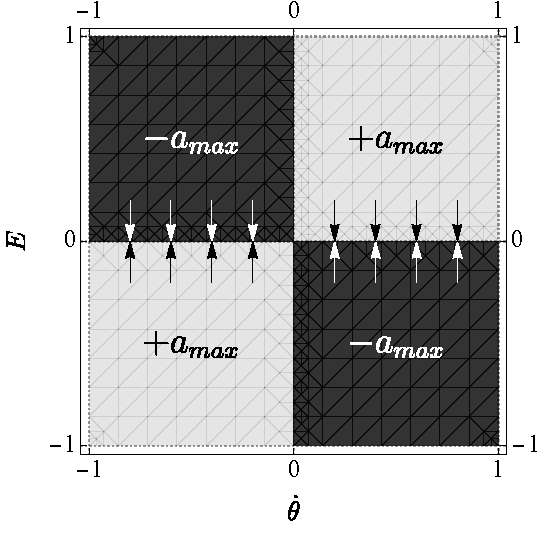
\includegraphics[width=\textwidth]{assets/energy-control1}
        \caption{aaaaa}
    \end{subfigure}
    \hfill
    \begin{subfigure}[b]{0.48\textwidth}
        \centering
        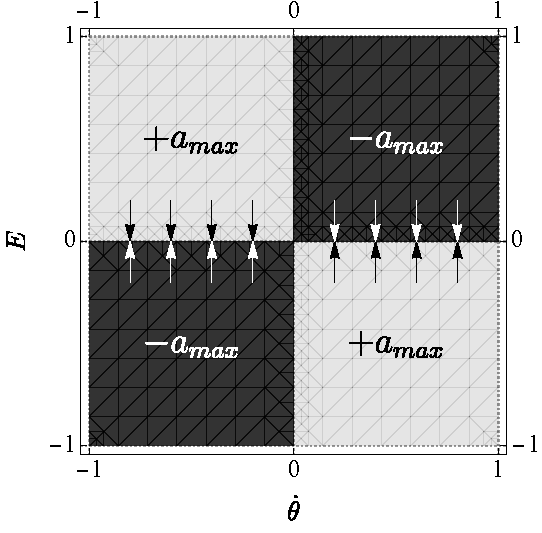
\includegraphics[width=\textwidth]{assets/energy-control2}
        \caption{bbbbb}
    \end{subfigure}
    \caption{Schema del sistema.} %todo
    \label{fig:energy-control}
\end{figure}

\subsection{Funzione di controllo di Ljapunov}
\paragraph{Si può fare di meglio,} impiegando una CLF per ricavare una strategia di controllo. Questo permette sia di avere una strategia di controllo smooth, sia di dimostrare rigorosamente che il sistema raggiungerà l'equilibrio cercato, grazie ai teoremi ??\todo{qui dovrò citare teoremi scritti prima su controllabilità con lyapunov}.
Devo trovare una strategia di controllo $a$ e una funzione di Lyapunov $V$ che rispettino le condizioni di [riferimento alla definizione di funzione di lyapunov \todo{teoria}].
Per cercare $a$ mi ispiro alle considerazioni fatte a fine paragrafo \ref{subsec:energia-pendolo}. La funzione che si presta di più è la tangente tangente iperbolica, per via dell'effetto soglia:
\begin{equation}
    a = a_{\max} \tanh(E \dot \theta \cos \theta).
    \label{eq:control-strategy-test}
\end{equation}
Questa strategia è schematizzata in figura \ref{fig:energy-control-smooth}.
\begin{figure}
    \centering
    \begin{subfigure}[b]{0.48\textwidth}
        \centering
        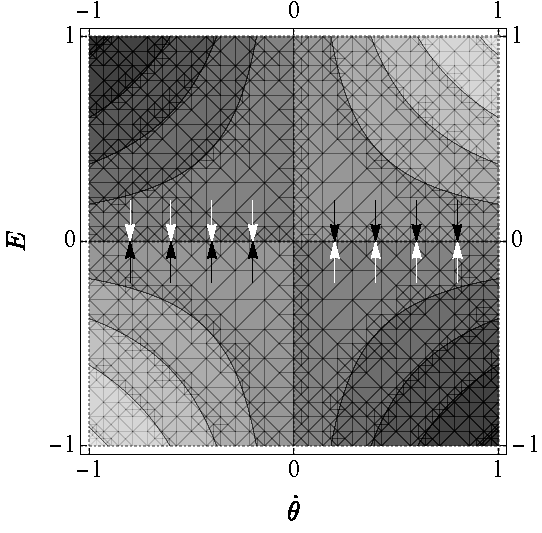
\includegraphics[width=\textwidth]{assets/energy-control3}
        \caption{aaaaa}
    \end{subfigure}
    \hfill
    \begin{subfigure}[b]{0.48\textwidth}
        \centering
        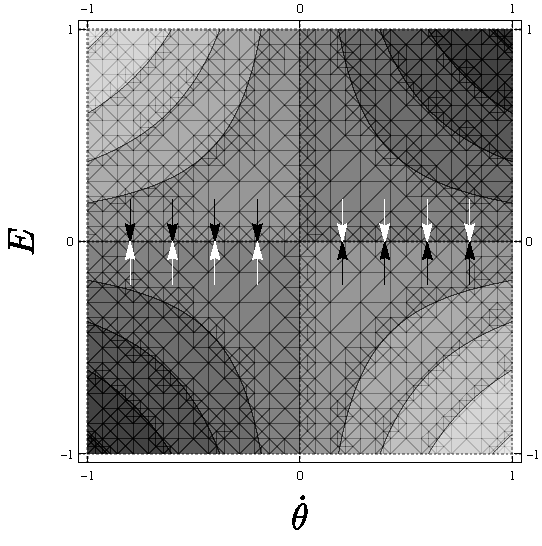
\includegraphics[width=\textwidth]{assets/energy-control4}
        \caption{bbbbb}
    \end{subfigure}
    \caption{Schema del sistema.} %todo
    \label{fig:energy-control-smooth}
\end{figure}

Ora, se definisco $V$ come:
\begin{equation}
    V = \frac 1 2 E^2.
    \label{eq:lyapunov-energy}
\end{equation}
È facile dimostrare che ho trovato una CLF. Infatti, se calcolo la detivata di $V$ e sostituisco l'espressione di $a$ appena definita:
\begin{equation}
    \begin{aligned}
        \totald t V &= \totald t \left( \frac 1 2 \dot E^2\right) \\
        &=  E \dot E \\
        &=  E (-maL \dot \theta \cos \theta) \\
        &= -mLE\dot \theta \cos \theta \cdot a_{\max} \tanh(E \dot \theta \cos \theta).
    \end{aligned}
    \label{eq:lyapunov-energy}
\end{equation}
Per dimostrare che questa è una CLF devo mostrare che $V'(t) < 0 q.o.$ e ciò è banale visto che la tangente iperbolica preserva il segno. Di conseguenza la funzione è negativa a patto che:
\begin{itemize}
    \item $\dot \theta \neq 0$
    \item $\cos \theta \neq 0$
\end{itemize}
tuttavia, nessuna di queste configurazioni è stabile per il sistema\footnote{$\dot \theta = 0$ è stabile se $\theta = \{0, \pi\}$, ma $\theta = 0$ è il punto a cui vogliamo arrivare e $\theta = \pi$ è il punto di partenza; basta quindi fornire un impulso iniziale al sistema e questo inizierà a muoversi.}, quindi possiamo affermare che $V$ tenderà a zero e l'angolo tenderà a $\theta = 0$.
È opportuno sottolineare che questa strategia non tiene in considerazione la posizione del carrello lungo la rotaia.
È quindi necessario passare alla strategia \ref{sec:strategia-stabilizzazione}
una volta che il pendolo raggiunge la verticale.
\section{Stima dei parametri del sistema nel mondo reale}
Non tutti i parametri descritti in tabella \ref{tab:parametri} sono calcolabili facilmente. In particolare, mi sono sconosciuti:
\begin{itemize}
    \item I parametri del motore.
    \item Il momento d'inerzia del pendolo.
\end{itemize}
In questa sezione userò i dati raccolti dal sistema reale per ottenere una stima di questi parametri.
Anche qui, mi conviene separare lo studio del pendolo dallo studio del motore.

\subsection{Parametri del pendolo}
La massa del pendolo si può misurare direttamente con una bilancia.
Anche la posizione del centro di massa è facile da trovare, bilanciando
il pendolo su un supporto e misurando la distanza tra questo e l'estremità.
Il momento d'inerzia è difficile da calcolare direttamente, visto che il
pendolo che ho usato è stato realizzato tramite la stampa 3d e, di conseguenza,
è estremamente disomogeneo all'interno; si può ricavare misurando
il periodo $\tau_{osc}$ di oscillazione del pendolo.
L'equazione del moto, nel regime delle piccole oscillazioni, è:
\begin{equation*}
    J \ddot \theta = mgL \sin \theta \approx mgL \theta
\end{equation*}
da cui
\begin{align}
    \omega &= \sqrt{\frac {m g L} J},\\
    \tau_{osc} &= \frac{2\pi}\omega = 2\pi \sqrt{\frac J {mgL}}.
    \label{eq:tau-osc}
\end{align}
La~\eqref{eq:tau-osc} permette di ricavare $J$ e fornisce una scala
di tempo per il sistema.


\subsection{Parametri del motore}
\label{subsec:parametri-motore}
Per determinare i parametri del motore, osservo come si comporta il sistema del solo
carrello, quando applico una \ddp $u$ costante ai capi del motore.
L'equazione che regola il comportamento del motore è la \eqref{eq:caratteristica-motore}.
Se scollego il pendolo dal carrello, l'espressione per la forza $f$
esercitata dal motore è data dalla legge di Newton:
\begin{equation}
    f = M \ddot q.
    \label{eq:newton-motore}
\end{equation}
Ora considero la sostituzione
\begin{equation}
    \begin{aligned}
    \dot q \mapsto v \\
    \ddot q \mapsto \dot v
    \end{aligned}
    \label{eq:sostituzione-motore}
\end{equation}
e inserendo \eqref{eq:newton-motore} e\eqref{eq:sostituzione-motore} dentro a \eqref{eq:caratteristica-motore}
ottengo l'equazione di una legge esponenziale:
\begin{equation*}
    \dot v = \frac{u - B v} {Am}.
\end{equation*}
Fisso la condizione iniziale $v(0) = 0$ e ottengo la soluzione:
\begin{equation}
    v(t) = \frac u B \left(1 - e^{-\frac B {Am} t}\right).
    \label{eq:equazione-fit-motore}
\end{equation}
I parametri $A$ e $B$ sono costanti quindi, variando $u$, mi aspetto di trovare
una famiglia di curve con cui fittare la \eqref{eq:equazione-fit-motore}.

In questa trattazione ho trascurato l'attrito tra carrello e rotaia.
Visto che il carrello scorre sulla rotaia attraverso dei cuscinetti,
l'attrito si può approssimare come costante.
Nel paragrafo ?? \todo{ref sezione risultati} mostrerò che in effetti questo attrito
è trascurabile.
\todo {traduci?}
Non è trascurabile invece il \emph{cogging torque} $\tau_c$ del motore,
dovuto all'interazione tra i magneti permanenti e le armature. $\tau_c$ ha
l'andamento descritto in figura \ref{fig:cogging} ed è predominante quando $\omega$ è
piccola.
L'approccio che ho usato per ridurne l'effetto è descritto nel paragrafo ?? \todo{anche qui paragrafo}.

%fixme i have no idea what this does but i used it so that the figure next doesn't span across
the whole page.
\makeatletter
\setlength{\@fptop}{0pt}
\makeatother

\begin{figure}[t]
    \centering
    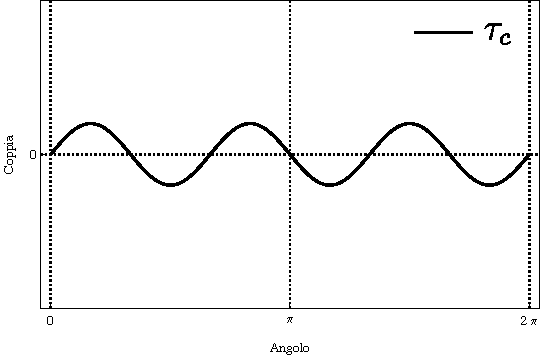
\includegraphics{assets/cogging-torque}
    \caption[Cogging torque]{Cogging toque del motore.}
    \label{fig:cogging}
\end{figure}

            \title{Risultati}
\maketitle
\label{sec:conclusions}

\paragraph{Introduzione.}
bla bla

\section{Parametri del sistema}
Il valore numerico di tutti i parametri d'interesse per il sistema è riportato
in \autoref{tab:parametri-numerici}.
Ho misurato direttamente la maggior parte dei
parametri, esclusi quelli relativi al motore.
Per
determinare questi ultimi, ho seguito il procedimento spiegato nel
paragrafo~\ref{subsec:parametri-motore}.

\bgroup
\renewcommand{\tabularxcolumn}[1]{>{\arraybackslash}m{#1}}
\renewcommand\arraystretch{1.5}
\begin{table}[H]
    \centering
\begin{tabular}{| gc | c | }
        \noalign{\hrule height 2pt}
        \rowcolor{Black}%
        \multicolumn{1}{=c}{\rowstyle{\bfseries\sffamily \color{White}} Parametro} & \multicolumn{1}{+c}{ Valore} \\
        \hline
        $g$ & $9,8 \sfrac m {s^2}$ \\
        \hline
        $M$ & $210g$ \\
        \hline
        $m$ & $22g$ \\
        \hline
        $l$ & $11.8cm$ \\
        \hline
        $I$ & $0.36\sfrac g {m^2}$ \\
        \hline
        $A$ & $28.5 N^{-1}$ \\
        \hline
        $B$ & $120 \sfrac s m$ \\
        \hline
        \noalign{\hrule height 2pt}
    \end{tabular}
    \caption{Parametri numerici del sistema.}
    \label{tab:parametri-numerici}
\end{table}
\egroup

\subsection{Parametri del motore}
\label{subsec:parametri-motore}
Per determinare i parametri del motore osservo il comportamento del solo
carrello quando applico un segnale $u$ costante al motore.
L'equazione che regola il comportamento del motore è la~\eqref{eq:caratteristica-motore}.
L'espressione per la forza $f$
esercitata dal motore è data dalla legge di Newton:
\begin{equation}
    f = M \ddot q.
    \label{eq:newton-motore}
\end{equation}
Inserisco la~\eqref{eq:newton-motore} nella~\eqref{eq:caratteristica-motore}
e applico la sostituzione
\begin{equation*}
    \left\{
    \begin{aligned}
        \dot q \mapsto v \\
        \ddot q \mapsto \dot v
    \end{aligned}
    \right.
    _.
    \label{eq:sostituzione-motore}
\end{equation*}
Ottengo
\begin{equation*}
    \dot v = \frac{u - B v} {Am}.
\end{equation*}
Fisso la condizione iniziale $v(0) = 0$ e ottengo
\begin{equation}
    v(t) = \frac u B \left(1 - e^{-\frac B {Am} t}\right).
    \label{eq:equazione-fit-motore}
\end{equation}
I parametri $A$ e $B$ sono costanti quindi, variando $u$, mi aspetto di trovare
una famiglia di curve con cui svolgere un \emph{fit} per la~\eqref{eq:equazione-fit-motore}.

In \autoref{fig:motor-vmax-fit} ho riportato i dati delle velocità in funzione di
$u$ e del tempo $t$.
Chiamo $v_\infty(u)$ il limite della
curva~\eqref{eq:equazione-fit-motore} per $t \to +\infty$.
I valori di
$v_\infty(u)$ sono ottenuti da una media delle velocità oltre un certo tempo.
Nella \autoref{fig:motor-vmax-fit} una linea verticale delimita i punti su cui è
stata eseguita la media e a sinistra sono riportati i valori numerici delle $v_\infty(u)$.

\begin{figure}[H]
    \centering
    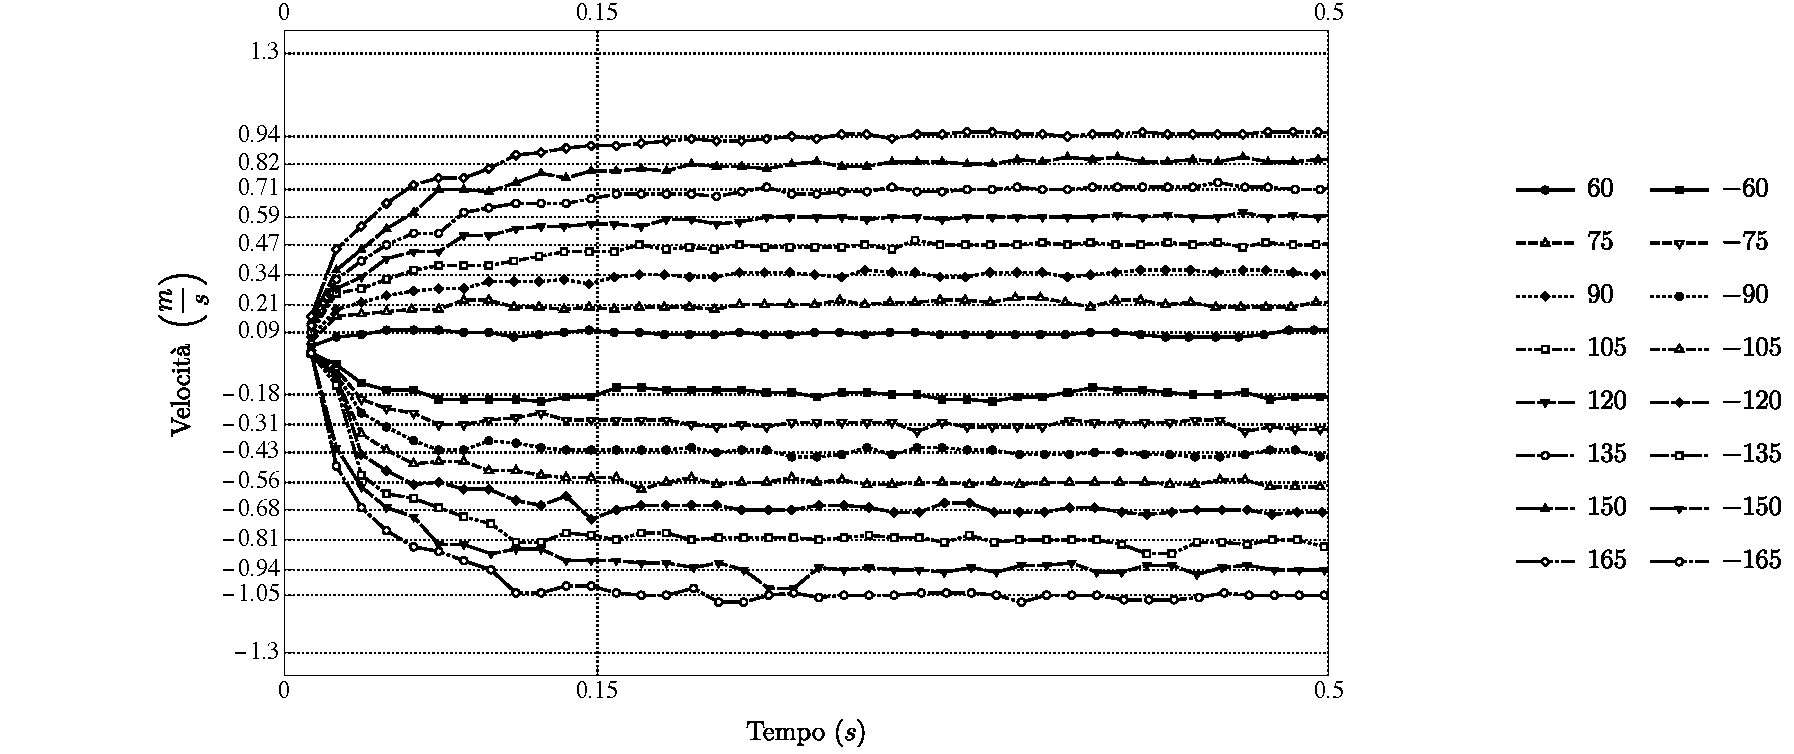
\includegraphics[width=\textwidth]{assets/motor-vmax-fit}
    \caption[Dati per stimare i parametri del motore]{Dati usati
    per stimare i parametri del motore. A sinistra sono riportati i valori
    a cui tende la velocità del carrello per un certo segnale di input al
    motore, calcolati come la media dei punti dopo il tempo $t = .15s$.
    Il valore di $u$ per ogni serie di dati è riportato in legenda, espresso
    in $(PWM)$. Vale $1 (PWM) = \sfrac {12}{255}V$.
    }
    \label{fig:motor-vmax-fit}
\end{figure}

Da un fit lineare delle $v_\infty(u)$ ricavo il parametro $B$ come inverso
della pendenza della retta
\begin{equation}
    v_\infty(u) = m u + q.
    \label{eq:vinfmuq}
\end{equation}
Il risultato del fit è riportato in \autoref{fig:motor-offset}; il valore
numerico di $B$ è
\begin{equation*}
    B = 120 \sfrac s m.
\end{equation*}

\begin{figure}[H]
    \centering
    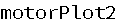
\includegraphics[width=\textwidth]{assets/motor-offset}
    \caption[Fit lineare delle velocità asintotiche del carrello]{
    Fit lineare delle $v_{\infty}(u)$. Le velocità negative e quelle positive
    giacciono su due rette che hanno stessa pendenza ma diversa intercetta.
    La discrepanza è dovuta all'attrito tra carrello e rotaia.
    }
    \label{fig:motor-offset}
\end{figure}

Infine ricavo $A$ da un fit esponenziale sulla famiglia di curve~\eqref{eq:equazione-fit-motore}. Il risultato è riportato in \autoref{fig:motor-expo-fit}; il valore
numerico di $A$ è
\begin{equation*}
    A = 28.5 N^{-1}.
\end{equation*}

\begin{figure}[H]
    \centering
    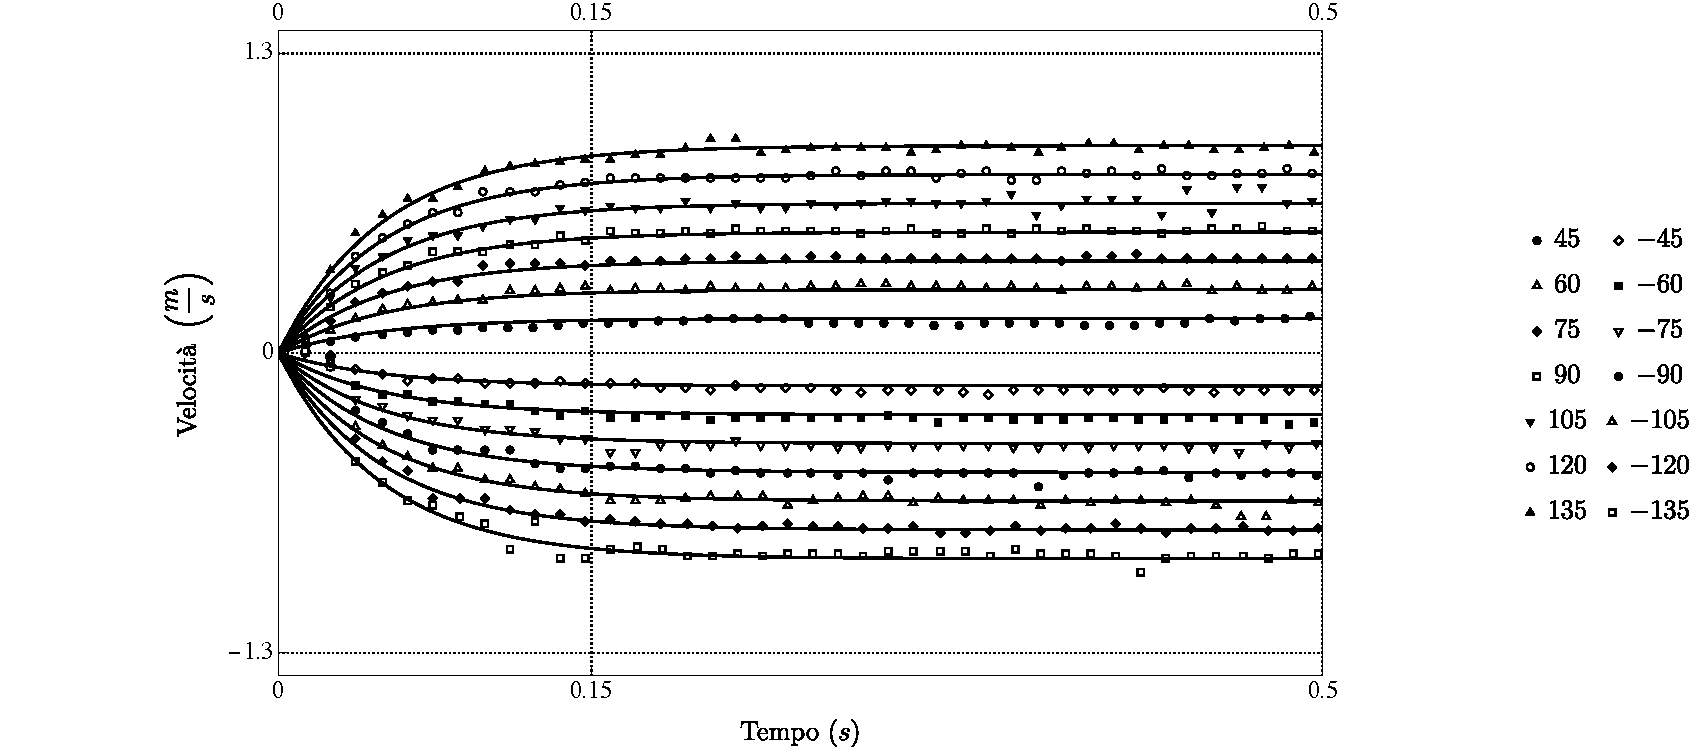
\includegraphics[width=\textwidth]{assets/motor-expo-fit}
    \caption[Fit esponenziale per i parametri del motore]{
    Fit esponenziale per trovare il parametro A del motore.
    }
    \label{fig:motor-expo-fit}
\end{figure}

Nel mio modello non compaiono attriti.
In realtà, il carrello scorre su dei cuscinetti a sfera,
quindi mi aspetto sia presente un attrito costante tra esso e la rotaia.
Fa parte degli attriti anche la \emph{coppia d'impuntamento} $\tau_c$ del motore,
dovuta all'interazione tra i magneti permanenti e le armature. $\tau_c$ ha
l'andamento descritto in \autoref{fig:cogging} ed è predominante quando $\omega$ è
piccola.
Correggo entrambi gli attriti aggiungendo un offset $u_{\min} $ a $u$, dato dall'intercetta della~\eqref{eq:vinfmuq}.

 
%fixme i have no idea what this does but i used it so that the figure next doesn't span across
%the whole page.
%\makeatletter
%\setlength{\@fptop}{0pt}
%\makeatother

\begin{figure}[H]
    \centering
    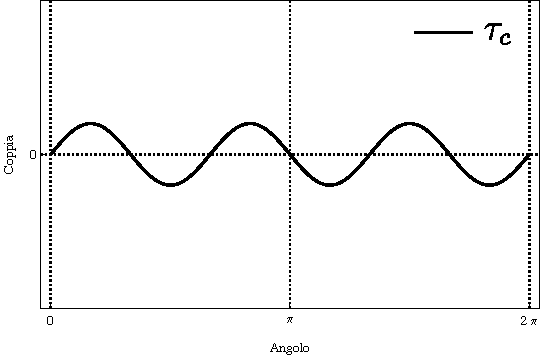
\includegraphics{assets/cogging-torque}
    \caption[Coppia d'impuntamento]{Andamento qualitativo della coppia d'impuntamento
    di un motore DC, in funzione dell'angolo del perno centrale.}
    \label{fig:cogging}
\end{figure}

\section{Risultati della stabilizzazione}
\autoref{subsec:comportamento-asintotico}
\section{Risultati dello swing-up}
\section{Questo esperimento come metodo didattico}

        \appendix           % "Chapter" is renamed "Appendix"
        \appendixpage       % Similar to \part*{Appendices}, but appears in TOC

            \chapter{The First Appendix}
\label{app:first-app}
\kant[20-21] % Dummy text
\section{First Section}
\kant[22]    % Dummy text
\section{Second Section}
\kant[23-24] % Dummy text


    %\bibliographystyle{unsrt} % We choose the "plain" reference style
    %\bibliography{dpicRefs}
\end{document}
